\documentclass[lettersize,journal]{IEEEtran}
\usepackage{amsmath,amsfonts,amssymb}
\usepackage{algorithmic}
\usepackage{algorithm}
\usepackage{array}
\usepackage[caption=false,font=normalsize,labelfont=sf,textfont=sf]{subfig}
\usepackage{textcomp}
\usepackage{stfloats}
\usepackage{url}
\usepackage{verbatim}
\usepackage{graphicx}
\usepackage{cite}
\usepackage{booktabs}
\usepackage{multirow}
\hyphenation{op-tical net-works semi-conduc-tor IEEE-Xplore}
\renewcommand{\algorithmicrequire}{\textbf{Input:}}
\renewcommand{\algorithmicensure}{\textbf{Output:}}
\newcommand{\Dmax}{D^{\max}}
\newcommand{\Amin}{A^{\min}}

\begin{document}

\title{UT-SMART: Uncertainty-Aware Twin-Assisted Semantic Multi-Agent Edge Intelligence for Connected Autonomous Underwater Vehicles}

\author{Manimurugan~Shanmuganathan,~\IEEEmembership{Senior~Member,~IEEE,}
        P.~Karthikeyan,
        Ahmed~Aljuhani,
        and~Alireza~Jolfaei,~\IEEEmembership{Senior~Member,~IEEE}%
\thanks{Manuscript received XX; revised XX. (Corresponding author: Manimurugan Shanmuganathan.)}%
\thanks{Manimurugan Shanmuganathan and Ahmed Aljuhani are with the Faculty of Computers and Information Technology, University of Tabuk, Tabuk 71491, Saudi Arabia (e-mail: mmurugan@ut.edu.sa; a\_aljuhani@ut.edu.sa).}%
\thanks{P. Karthikeyan is with the School of Computer Science and Engineering, RV University, Bengaluru 560059, India (e-mail: karthikeyanp@rvu.edu.in).}%
\thanks{Alireza Jolfaei is with the College of Science and Engineering, Flinders University, Adelaide, Australia (e-mail: alireza.jolfaei@flinders.edu.au).}}

\markboth{IEEE Transactions on Vehicular Technology, Special Issue on Edge Intelligence and In-Network Computing for Connected AUVs}%
{Shanmuganathan \MakeLowercase{\textit{et al.}}: UT-SMART: Uncertainty-Aware Twin-Assisted Semantic Multi-Agent Edge Intelligence}

\maketitle

\begin{abstract}
Connected autonomous underwater vehicles (AUVs) can act as mobile edge servers for seabed sensors, but kilobit-per-second acoustic links, stale channel knowledge and compromised vehicles undermine conventional offloading. This paper proposes UT-SMART, an uncertainty-aware, twin-assisted, semantic multi-agent edge-intelligence framework. Seabed sensors extract task-relevant features at four compression levels, a form of semantic in-network computing. Each AUV keeps a Bayesian digital twin of its links that tracks its own prediction uncertainty, probes a link only when it is both uncertain and about to be used, and evaluates every candidate action with mean and pessimistic delay predictions. A parameter-shared constrained multi-agent proximal policy optimization (MAPPO) policy selects the compression level and the executor (own AUV, neighbour AUV or surface gateway) under mission-specific deadline, accuracy and value-of-information constraints. Beta-reputation trust and event-triggered state sharing are built into the policy. In simulations with Thorp--Urick acoustic channels, shadowing, outages and short-range optical links, evaluated over 10 seeds, UT-SMART completes 98.9\% of tasks when a gateway is available. This matches a MAPPO baseline while cutting control traffic by 89\% and twin prediction error by 34\%, and it far outperforms raw offloading (33.7\%) and delay--energy best response (20.3\%). When inference must stay on AUVs and one vehicle is compromised, UT-SMART completes 89.2\% of tasks against 75.8\% for MAPPO and reduces accepted corrupted results from 11.5\% to 2.2\%.
\end{abstract}

\begin{IEEEkeywords}
Autonomous underwater vehicles, edge intelligence, in-network computing, semantic communication, digital twin, uncertainty quantification, multi-agent reinforcement learning, trust management, underwater acoustic networks.
\end{IEEEkeywords}

%======================================================================
\section{Introduction}
\subsection{Background and Motivation}
\IEEEPARstart{C}{onnected} autonomous underwater vehicles (AUVs) are becoming mobile edge servers for the Internet of Underwater Things. They collect sonar, image and environmental data from seabed sensors, run inference close to the data and relay results to surface gateways~\cite{yang2021survey,dai2022survey,lin2025madac}. Underwater acoustic links are the main bottleneck. They offer a few kilobits per second, propagate at about 1500~m/s, suffer frequency-dependent absorption, and fade or drop out as vehicles move~\cite{song2025dtna,xu2025stgr,shu2026offload,stojanovic2007capacity}. Optical links are fast but reach only tens of metres. Sending raw data to an edge server, the default in terrestrial mobile edge computing (MEC)~\cite{mao2017mec,pang2020sagin,chen2025ios,su2020maritime}, therefore overloads the acoustic medium and drains the limited batteries of seabed nodes.

Recent work has tackled parts of this problem. Game-theoretic offloading balances delay and energy among underwater sensors, AUVs and buoy servers~\cite{shu2026offload}. Digital twins (DTs) of underwater acoustic sensor networks improve resource allocation and accelerate multi-agent training~\cite{song2025dtna}. Spatial-temporal graph models make multi-vehicle routing more reliable~\cite{xu2025stgr}. Multi-agent reinforcement learning (MARL) plans AUV data-collection paths with value-of-information (VoI) awareness~\cite{lin2025madac}. In-network computing (INC) pushes processing into the forwarding path to cut latency~\cite{wu2024inc,hong2024cnc}. Security surveys show that AUV systems face spoofing, jamming, data poisoning and compromised nodes~\cite{ahmad2026survey}. From this literature we identify five gaps that no single framework closes.

\begin{enumerate}
\item \emph{Communication, computation and intelligence are optimized separately.} Joint offloading schemes minimize delay and energy~\cite{shu2026offload,chen2025ios} but do not treat inference quality as a constraint. A cheap, highly compressed transmission can meet a deadline and still fail the mission.
\item \emph{Twins assume their state is accurate.} Underwater observations are delayed and sparse. A twin that predicts from stale link estimates can recommend offloading over a link that has already faded~\cite{song2025dtna}.
\item \emph{Raw data still dominates the traffic.} Most underwater pipelines move raw sonar or image frames to an AUV or the cloud rather than extracting task-relevant semantics at the source~\cite{wu2024inc,dai2022survey}.
\item \emph{Multi-agent coordination is communication-hungry.} MARL schemes such as MADDPG variants assume frequent exchange of observations and state~\cite{lin2025madac}. Over acoustic links, that exchange competes with mission data.
\item \emph{Security is evaluated apart from decision-making.} Trust and anomaly detection are rarely part of the offloading policy itself~\cite{ahmad2026survey}. A compromised AUV that advertises free capacity can attract and corrupt critical tasks.
\end{enumerate}

\subsection{Related Work}
\subsubsection{Maritime and Underwater Edge Computing}
Su \emph{et al.}~\cite{su2020maritime} analysed maritime network connectivity and the edge computing capability of a cognitive big-data platform. Pang \emph{et al.}~\cite{pang2020sagin} proposed a space--air--ground integrated, MEC-based maritime network, and Chen \emph{et al.}~\cite{chen2025ios} surveyed edge computing architectures for the Internet of Ships. Dai \emph{et al.}~\cite{dai2022survey} reviewed integrated sensing, communication and computing for smart oceans across space, aerial, surface and underwater layers. These works establish edge computing at sea but focus mainly on surface and above-water links. Below the surface, the acoustic channel dominates every decision.

\subsubsection{Underwater Task Offloading}
Shu \emph{et al.}~\cite{shu2026offload} model AUV-assisted offloading with end--edge--cloud collaboration as a multi-sensor potential game. Their DA-GDUTO algorithm uses probabilistic parallel updates and lowers the weighted delay--energy cost by about 12\% over baselines. As in most offloading work, the objective is delay and energy; inference quality and mission value are not constraints.

\subsubsection{Digital Twins for Underwater Networks}
Song \emph{et al.}~\cite{song2025dtna} proposed DTNA, a layered architecture with local and global twins of underwater acoustic sensor networks. It supports resource allocation (RAPD), collaborative MARL training (CMFD) and task-oriented network slicing (TNSD). DTNA shows that twins can speed up training and improve timeliness. Its twin, however, does not quantify its own uncertainty or decide when it is reliable enough to act on.

\subsubsection{Multi-AUV Coordination and Routing}
Yang \emph{et al.}~\cite{yang2021survey} surveyed AUV formation and found that communication capability is the least mature dimension. Zhang \emph{et al.}~\cite{zhang2025dfxtna} designed a distributed fixed-time neurodynamic algorithm for multi-AUV escorting. Xu \emph{et al.}~\cite{xu2025stgr} proposed STGR, which combines a spatial-temporal graph of link quality and connectivity duration with Q-learning forwarder selection. Lin \emph{et al.}~\cite{lin2025madac} presented MADAC, a software-defined MARL framework (MADDPG with similarity attention) for VoI-aware multi-AUV data collection. In the machine-learning literature, MADDPG~\cite{lowe2017maddpg} introduced centralized critics with decentralized actors, and TarMAC~\cite{das2019tarmac} learns what to communicate and to whom. These methods coordinate agents well but assume regular, cheap exchange of state, actions or messages, which acoustic links cannot provide.

\subsubsection{Learning-Based Offloading and Edge Inference}
Mao \emph{et al.}~\cite{mao2017mec} surveyed MEC with a focus on joint radio and computational resource management. Huang \emph{et al.}~\cite{huang2020droo} proposed DROO, a deep reinforcement learning framework that learns binary offloading decisions under time-varying wireless channels. Kang \emph{et al.}~\cite{kang2017neurosurgeon} showed that partitioning DNN computation between mobile devices and the cloud at layer granularity reduces both latency and device energy. Shao \emph{et al.}~\cite{shao2022taskoriented} formulated task-oriented communication for edge inference with an information-bottleneck framework that trades feature informativeness against rate, and Xie \emph{et al.}~\cite{xie2021deepsc} proposed DeepSC, a deep-learning semantic communication system that is robust at low SNR. These works assume radio links with millisecond latency and do not face the kilobit-per-second, second-scale propagation regime of underwater acoustics, which makes source-side semantic compression far more consequential.

\subsubsection{In-Network and Convergent Computing}
Wu \emph{et al.}~\cite{wu2024inc} embedded computation into programmable network devices and cut latency for control and event-processing workloads. Hong \emph{et al.}~\cite{hong2024cnc} proposed an intelligence-endogenous ``CNC brain'' that matches computing supply and demand with deep reinforcement learning. Both are terrestrial. We carry the in-network idea to the seabed: sensor nodes extract compact, task-relevant features before data enters the acoustic medium.

\subsubsection{Security of Autonomous Vehicle Systems}
Ahmad \emph{et al.}~\cite{ahmad2026survey} surveyed cyber threats across air, ground and underwater autonomous systems, including spoofing, jamming, denial of service, data poisoning and compromised nodes, and showed that they can propagate across domains. Trust management is usually a separate monitoring layer. UT-SMART instead places a trust score inside the task-allocation policy.

Table~\ref{tab:related} summarizes the gap. To our knowledge, no prior underwater framework jointly handles semantic compression, twin uncertainty, inference-quality constraints, communication-efficient MARL and trust.

\begin{table*}[!t]
\centering
\caption{Comparison With Representative Related Work}
\label{tab:related}
\begin{tabular}{@{}lcccccc@{}}
\toprule
Work & \shortstack{Joint\\comm.--comp.} & \shortstack{Inference\\quality / VoI} & \shortstack{Twin with\\uncertainty} & \shortstack{In-network\\semantics} & \shortstack{Low-overhead\\MARL} & \shortstack{Trust in\\policy}\\
\midrule
Shu \emph{et al.}~\cite{shu2026offload} & Yes & No & No & No & No (game) & No\\
Song \emph{et al.}~\cite{song2025dtna} & Yes & Task slicing & Twin, no uncertainty & No & No & No\\
Xu \emph{et al.}~\cite{xu2025stgr} & Routing only & No & No & No & Q-learning & No\\
Lin \emph{et al.}~\cite{lin2025madac} & Data collection & VoI & No & No & No & No\\
Wu \emph{et al.}~\cite{wu2024inc} & Yes & No & No & Yes (terrestrial) & No & No\\
\textbf{UT-SMART} & \textbf{Yes} & \textbf{Accuracy + VoI + deadline} & \textbf{Yes} & \textbf{Yes} & \textbf{Event-triggered} & \textbf{Yes}\\
\bottomrule
\end{tabular}
\end{table*}

\subsection{Contributions and Organization}
This paper proposes \emph{UT-SMART} (Uncertainty-aware Twin-assisted Semantic Multi-Agent Reinforcement learning with Trust). For every sensing task, UT-SMART decides how strongly the sensor compresses the data and which node runs inference: the cluster AUV, a neighbouring AUV or the surface gateway. The main contributions are as follows.
\begin{itemize}
\item \emph{A mission-aware joint formulation.} We model a 3-D sensor field served by patrolling AUVs over Thorp--Urick acoustic links with log-normal shadowing, Markov outages and short-range optical links. Tasks carry mission-specific deadlines, minimum inference accuracy and VoI. The decision problem is a constrained Markov decision process (CMDP) that couples semantic compression, link scheduling, computing and inference quality.
\item \emph{An uncertainty-aware digital twin.} Each AUV keeps a Bayesian (Kalman) twin of its links that tracks both the estimate and its posterior variance. The twin evaluates every candidate action with mean and lower-confidence-bound delay predictions, and it probes a link only when that link is about to be used and its uncertainty exceeds a threshold (on-demand synchronization).
\item \emph{Semantic in-network computing.} Sensors run lightweight encoders at four compression levels ($1\times$, $4\times$, $16\times$, $64\times$). Each level trades transmission time and energy against a mission-dependent accuracy loss.
\item \emph{Trust-aware, communication-efficient MARL.} A parameter-shared constrained MAPPO policy runs locally on each AUV and scores the twin's what-if predictions. A centralized critic and Lagrangian dual ascent enforce the deadline and accuracy constraints. A Beta-reputation trust score built from delivery reliability, behavioural consistency and spot-checked result correctness enters the policy directly, and AUVs share state only when their load changes materially.
\item \emph{A reproducible evaluation.} We compare UT-SMART with four baselines over 10 seeds and four sweeps (sensor density, fleet size, channel variability and fraction of malicious AUVs) in two operating regimes, isolate each mechanism by ablation and map the twin's accuracy against its synchronization overhead.
\end{itemize}

The rest of the paper is organized as follows. Section~\ref{sec:model} presents the system model and the problem formulation. Section~\ref{sec:method} describes the UT-SMART framework. Section~\ref{sec:eval} reports the performance evaluation and discusses limitations, and Section~\ref{sec:concl} concludes the paper.

%======================================================================
\section{System Model and Problem Formulation}\label{sec:model}

\subsection{Network Scenario}
Fig.~\ref{fig:scenario} illustrates the considered scenario. The network has $M$ seabed sensor nodes spread over a $2\,\mathrm{km}\times2\,\mathrm{km}$ area at depths of 250--600~m. $N$ AUVs operate at 150--300~m, and a surface gateway with an edge server sits at the centre of the area. Sensors are grouped into $N$ clusters by proximity, and each cluster is served by one AUV. The AUV patrols a circle of radius $0.3L/\lceil\sqrt{N}\rceil$ around the cluster centre at 1.5~m/s, where $L=2$~km, and a spatially varying ocean current of up to 0.3~m/s pushes it off this path. Time is slotted with $\Delta=2$~s, and an episode lasts 500 slots (1000~s). The gateway reaches the mission control centre through satellite or cellular backhaul, which is fast compared with the acoustic segment and is therefore not modelled as a bottleneck. Each AUV carries an edge processor connected to acoustic and optical modems, imaging sonar, cameras and navigation sensors (inset of Fig.~\ref{fig:scenario}); it hosts the inference models, the digital twin, the decision policy and the trust module.

\begin{figure*}[!t]
\centering
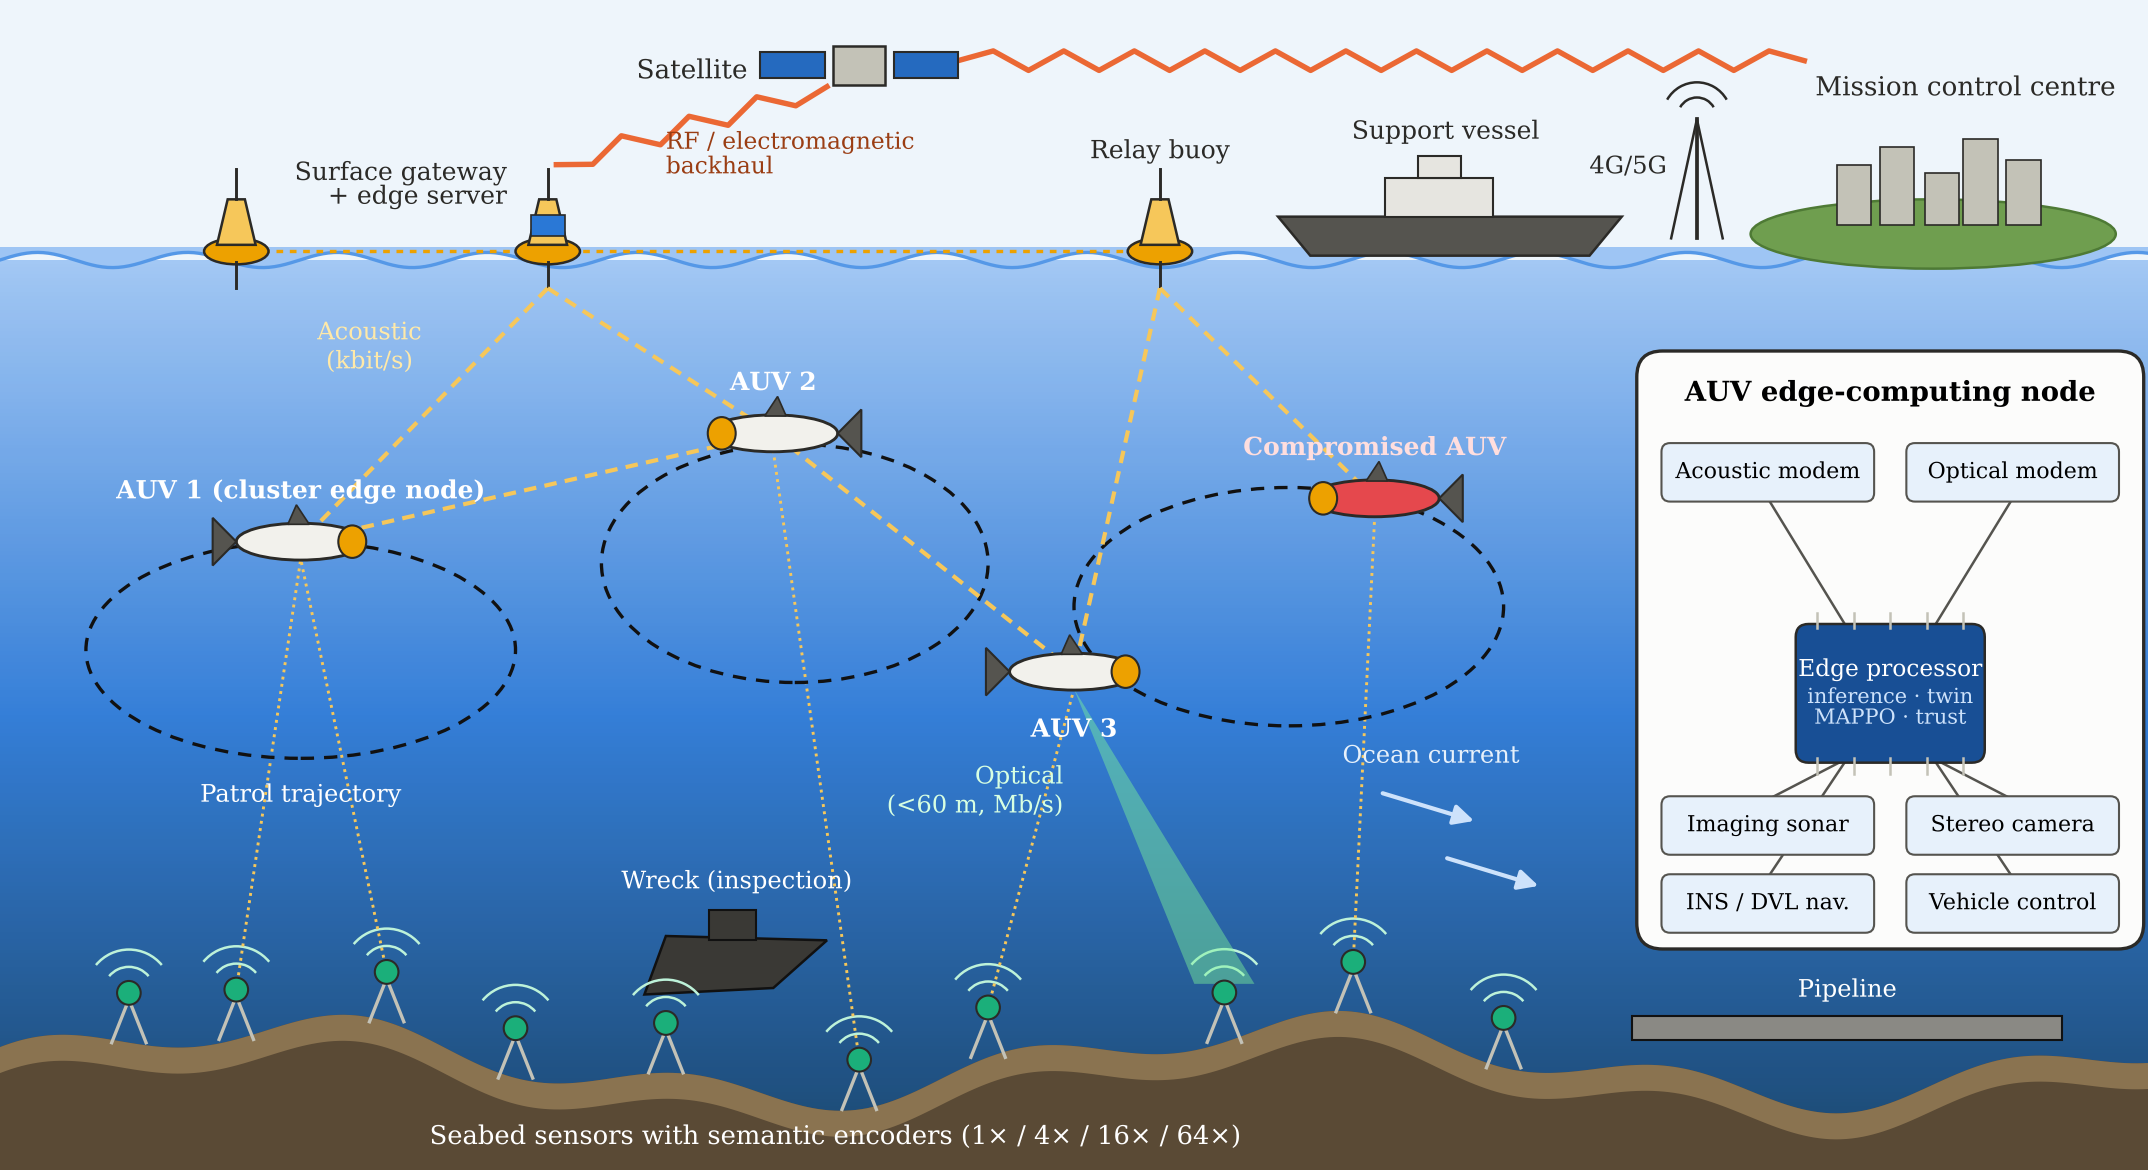
\includegraphics[width=\textwidth]{fig_scenario.png}
\caption{Connected-AUV edge-intelligence scenario. Seabed sensors encode data semantically and send it over short-range acoustic or optical links to patrolling AUVs; AUVs run inference or forward tasks to neighbours or to the surface gateway; the gateway connects to mission control by satellite or cellular backhaul. One AUV is compromised. Inset: the AUV edge-computing node.}
\label{fig:scenario}
\end{figure*}

\subsection{Acoustic and Optical Channels}
For a link of length $d$ (m) at carrier frequency $f$ (kHz), the path loss in dB is
\begin{equation}
A(d,f) = 10k\log_{10} d + \frac{d}{1000}\,\alpha(f),\qquad k = 1.5,
\end{equation}
where the absorption $\alpha(f)$ in dB/km follows Thorp's formula~\cite{stojanovic2007capacity}
\begin{equation}
\alpha(f) = \frac{0.11 f^2}{1+f^2} + \frac{44 f^2}{4100+f^2} + 2.75\cdot 10^{-4} f^2 + 0.003 .
\end{equation}
The ambient noise $N(f)$ is the sum of Urick's turbulence, shipping (activity $s=0.5$), wind ($w=5$~m/s) and thermal components, as in~\cite{shu2026offload}. The instantaneous SNR of link $l$ in slot $t$ is
\begin{equation}
\gamma_l(t) = SL - A\big(d_l(t),f\big) - \big(N(f) + 10\log_{10} B\big) + \chi_l(t),
\end{equation}
\begin{equation}
\chi_l(t+1) = \rho\,\chi_l(t) + \sqrt{1-\rho^2}\,\sigma\, w_l(t),\quad w_l(t) \sim \mathcal{N}(0,1),
\end{equation}
where $\chi_l$ is log-normal shadowing with standard deviation $\sigma$ (default 4~dB) and slot correlation $\rho=0.97$, which gives a coherence time of roughly one minute. A two-state Markov process adds intermittent outages with $p_{\mathrm{off}}=0.004$ and $p_{\mathrm{on}}=0.05$ per slot. With ARQ, the effective goodput is
\begin{equation}
R_l(t) = \eta B \log_2\!\big(1+10^{\gamma_l/10}\big)\big(1-\mathrm{PER}(\gamma_l)\big),
\end{equation}
\begin{equation}
\mathrm{PER}(\gamma) = \big(1+e^{(\gamma-8)/1.5}\big)^{-1},
\end{equation}
and it is zero below 3~dB or during an outage. We use $f=12$~kHz, $B=4$~kHz and $\eta=0.4$, with source levels of 135~dB re~$\mu$Pa for sensors and 150~dB re~$\mu$Pa for AUVs and a sound speed of $v=1500$~m/s. When a sensor and its AUV are within 60~m, an optical link at 1~Mb/s replaces the acoustic one. The network therefore models when each medium is available instead of assuming continuous high-rate connectivity.

\subsection{Semantic Tasks and Missions}
Each sensor generates inference tasks as a Poisson process with rate $\lambda=1/600$~s$^{-1}$. A task belongs to one of three missions, each with its own deadline, VoI, minimum accuracy and raw size (Table~\ref{tab:missions}).

\begin{table}[!t]
\centering
\caption{Mission Profiles}
\label{tab:missions}
\setlength{\tabcolsep}{3.5pt}
\begin{tabular}{@{}lcccccc@{}}
\toprule
Mission & Share & $\Dmax$ (s) & VoI & $\Amin$ & Size (kbit) & $s_m$\\
\midrule
Disaster detection & 25\% & 90 & 3 & 0.80 & 150--300 & 0.8\\
Infrastructure inspection & 40\% & 240 & 2 & 0.88 & 300--600 & 1.3\\
Pollution monitoring & 35\% & 480 & 1 & 0.85 & 200--500 & 1.0\\
\bottomrule
\end{tabular}
\end{table}

Before transmitting, a sensor can run a lightweight semantic encoder, such as a MobileNetV3-style feature extractor followed by a task-oriented bottleneck. The encoder offers four levels $k\in\{0,1,2,3\}$ with compression ratios $\kappa_k\in\{1,4,16,64\}$ and costs $c_k\in\{0,100,150,200\}$ cycles per raw bit on a 100~MHz sensor processor. Compression reduces achievable accuracy by $\delta_k\in\{0,0.010,0.035,0.090\}$, scaled by the mission sensitivity $s_m$. A task compressed at level $k$ and executed on node $e$ therefore reaches accuracy
\begin{equation}
A(k,e) = A_e - s_m\,\delta_k,\qquad A_{\mathrm{AUV}} = 0.90,\; A_{\mathrm{GW}} = 0.95 .
\end{equation}
The gateway runs a larger model, so it is more accurate but sits behind a long acoustic uplink. These values are modelling assumptions in the range reported for compressed-feature and split inference; Section~\ref{sec:disc} discusses their calibration.

\subsection{Communication and Computing Pipeline}
The task's $b=S/\kappa_k$ bits enter the cluster's shared, half-duplex acoustic channel, served first-in first-out (FIFO) at the sensor's goodput. The executor is the cluster AUV ($e=0$), a neighbour AUV ($e=1$) or the gateway ($e=2$). For $e\in\{1,2\}$, the AUV forwards the bits through its outbound acoustic queue. Inference costs $2\times10^9$ cycles on raw input or $0.8\times10^9$ cycles on features, and 1.5 times as much at the gateway. AUVs compute at $F_{\mathrm{AUV}}=4\times10^9$~cycles/s and the gateway at $F_{\mathrm{GW}}=2\times10^{10}$~cycles/s. AUV executors send a 2-kbit result to the gateway, and a task completes when its result arrives there. The end-to-end delay is
\begin{multline}
D = \frac{c_k S}{f_s} + W^{\mathrm{ch}} + \frac{b}{R_s} + \frac{d_s}{v} \\
+ W^{\mathrm{up}} + \frac{b'}{R_{\mathrm{up}}} + \frac{d_{\mathrm{up}}}{v} + W^{\mathrm{cpu}}_e + \frac{C_{k,e}}{F_e},
\end{multline}
where the four groups are encoding, sensor-to-AUV transfer, forwarding (or result return) and inference; the $W$ terms are queueing delays; $b'$ is the forwarded payload; and $C_{k,e}$ is the inference load. Tasks still queued at their deadline are dropped.

\subsection{Energy}
Transmit power is $P_s=2$~W for sensors and $P_a=10$~W for AUVs. Computing costs $\beta_s=10^{-9}$~J/cycle on sensors~\cite{shu2026offload} and $\beta_a=5\times10^{-10}$~J/cycle on AUVs. The energy of a task is
\begin{equation}
E = c_k S\,\beta_s + P_s \frac{b}{R_s} + \mathbb{1}[e\neq 0]\,P_a\frac{b}{R_{\mathrm{up}}} + C_{k,e}\,\beta_e .
\end{equation}

\subsection{Threat Model}
A fraction $\rho_m$ of AUVs (default 20\%) is compromised. A compromised AUV corrupts 70\% of the inference results it produces (data poisoning) and silently drops 10\% of the tasks it receives. It also advertises zero backlog, which attracts tasks as in a sinkhole attack~\cite{ahmad2026survey}. Its relaying behaviour is otherwise normal, so it is not trivially detectable.

\subsection{Problem Formulation}\label{sec:problem}
We cast task handling as a CMDP~\cite{altman1999cmdp} in which each AUV is an agent that decides for the tasks of its own cluster.

\emph{State:} At slot $t$ the network state is
\begin{equation}
S_t = \{G_t, H_t, Q_t, E_t, C_t, T_t, \Theta_t\},
\end{equation}
where $G_t$ is the time-varying topology (AUV positions), $H_t$ the acoustic link states (shadowing and outage), $Q_t$ the four queue classes (cluster channel, AUV outbound, AUV CPU and gateway CPU), $E_t$ the energy spent, $C_t$ the computing capacity, $T_t$ the digital-twin estimates with their uncertainty and $\Theta_t$ the trust state. No agent observes $S_t$ directly. Agent $c$ sees a local observation $o_c$ built from its own queues, its twin's link posteriors, the last (possibly stale) advertised loads of its neighbours and the trust vector.

\emph{Action:} For a task $\tau$ arriving in cluster $c$, the agent chooses $a=(k,e)$ from $4\times3=12$ options: the compression level $k\in\{1\times,4\times,16\times,64\times\}$ and the executor $e$, which is the own AUV, the best-ranked neighbour AUV or the gateway. The neighbour is ranked by advertised backlog plus link distance; with the trust module on, AUVs whose trust is below $\tau_T$ are excluded. This decision fixes the sensor's encoder setting (semantic feature selection), the use of links and queues (communication allocation), offloading and cooperative assignment. Patrol trajectories are fixed in this study.

\emph{Utility:} A task succeeds when its result reaches the gateway by the deadline, its accuracy meets the mission minimum and the result is not corrupted:
\begin{equation}
\mathbb{1}^{\mathrm{succ}}_\tau = \mathbb{1}[D_\tau \le \Dmax_\tau]\;\mathbb{1}[A_\tau \ge \Amin_\tau]\;\mathbb{1}[\neg\,\mathrm{corrupt}_\tau].
\end{equation}
The per-task reward combines value, delay, energy and communication cost. It is a utility form of the weighted cost $w_1D+w_2E+w_3C+w_4L$, where $L=1-A$ is the mission inference loss:
\begin{multline}
r_\tau = \frac{V_\tau}{V_{\max}}\, A_\tau\, \mathbb{1}^{\mathrm{succ}}_\tau \Big(1 - w_1 \min\!\big(\tfrac{D_\tau}{\Dmax_\tau},1\big)\Big) \\
- w_2 \frac{E_\tau}{E_0} - w_3 \frac{B_\tau}{B_0} - w_5\,\mathbb{1}[\mathrm{corrupt}_\tau],
\end{multline}
where $B_\tau$ counts all acoustic bits, including retransmissions. We use $w_1=0.3$, $w_2=0.05$ ($E_0=20$~J, capped at $5E_0$), $w_3=0.03$ ($B_0=300$~kbit), $w_5=0.3$ and $V_{\max}=3$.

\emph{Constrained objective:}
\begin{align}
\max_{\pi}\;& J_r(\pi) = \mathbb{E}_{\pi}\Big[\textstyle\sum_{\tau} r_\tau\Big] \label{eq:obj}\\
\text{s.t.}\;& \Pr_\pi\big(D_\tau > \Dmax_\tau\big) \le \epsilon_D, \label{eq:c1}\\
& \Pr_\pi\big(A_\tau < \Amin_\tau\big) \le \epsilon_A, \label{eq:c2}
\end{align}
with $\epsilon_D=0.08$ and $\epsilon_A=0.02$. Energy, link capacity and computing capacity act as hard physical limits through the queueing model: offloaded bits wait for a channel, and expired tasks are dropped. Even in a static, fully observed form the problem contains generalized assignment and is NP-hard. Under partial and delayed observations it calls for a learned, decentralized policy, which we derive from the Lagrangian
\begin{equation}
\mathcal{L}(\pi,\boldsymbol\lambda) = J_r(\pi) - \lambda_D\big(P^{\mathrm{miss}}_\pi - \epsilon_D\big) - \lambda_A\big(P^{\mathrm{acc}}_\pi - \epsilon_A\big),\;\; \boldsymbol\lambda \ge 0 .
\end{equation}

%======================================================================
\section{Proposed UT-SMART Framework}\label{sec:method}

Fig.~\ref{fig:arch} shows the block diagram of UT-SMART, which is organized in three levels. Level~1 is local edge AI: sensors run semantic encoders and AUVs run inference. Level~2 is cooperative MARL: AUV agents make offloading and assignment decisions with a shared policy. Level~3 is twin intelligence: each AUV's digital twin predicts link states with uncertainty and evaluates candidate actions, and the gateway aggregates trust estimates.

\begin{figure*}[!t]
\centering
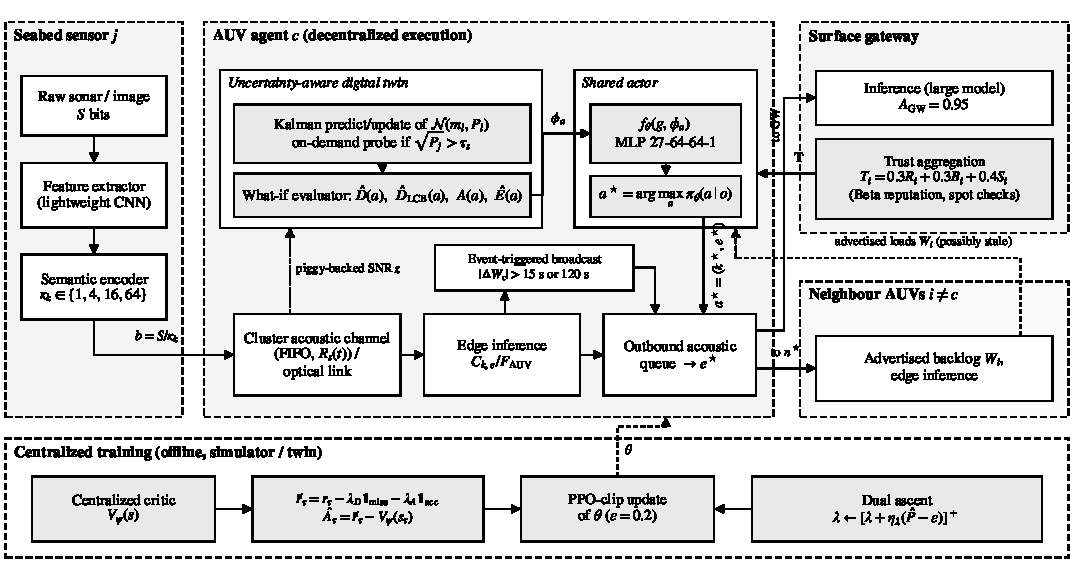
\includegraphics[width=\textwidth]{fig_arch.pdf}
\caption{Block diagram of UT-SMART. Each seabed sensor encodes its data at the compression level $\kappa_k$ chosen by the AUV agent. The AUV's uncertainty-aware digital twin (Kalman link posteriors with on-demand probing) evaluates all candidate actions, and the shared actor $f_\theta$ selects $a^\star=(k^\star,e^\star)$ using the twin's features $\phi_a$, the gateway's trust scores $\mathbf{T}$ and the neighbours' event-triggered load advertisements. Dashed lines denote control and measurement signals; the centralized critic and dual ascent are used only during offline training.}
\label{fig:arch}
\end{figure*}

\subsection{Uncertainty-Aware Digital Twin}
For every link $l$ it uses (sensor--AUV, AUV--gateway and AUV--AUV), the twin keeps a Gaussian posterior $\mathcal{N}(m_l,P_l)$ over the shadowing $\chi_l$; the deterministic path loss follows from known positions. In each slot the twin propagates the posterior with the AR(1) model
\begin{equation}
m_l \leftarrow \rho\, m_l,\qquad P_l \leftarrow \rho^2 P_l + (1-\rho^2)\,\sigma^2 .
\end{equation}
Every completed transmission gives a free (piggy-backed) SNR measurement $z$ with noise variance $R_m=1$~dB$^2$, which the twin fuses with a Kalman update:
\begin{equation}
K = \frac{P_l}{P_l + R_m},\quad m_l \leftarrow m_l + K (z - m_l),\quad P_l \leftarrow (1-K) P_l .
\end{equation}
Unlike learned predictors that need ensembles or Bayesian approximations to quantify their confidence~\cite{lakshminarayanan2017ensembles}, the Kalman twin carries its uncertainty $\sqrt{P_l}$ in closed form and uses it in two ways.

\emph{When to synchronize:} Under on-demand synchronization, when a task arrives at sensor $j$ and $\sqrt{P_j}>\tau_s$ (default 2.5~dB), the AUV sends a 512-bit probe exchange with priority before deciding. Links that are already reliable, or not about to be used, are never probed. Conventional periodic synchronization instead probes every link every $T_s$ seconds (default 60~s), whether or not the link is needed.

\emph{How far to trust a prediction:} For each of the 12 candidate actions, the twin runs a what-if evaluation of the delay pipeline in Section~\ref{sec:model}-D. It uses the current queue backlogs and two link-rate estimates: the posterior mean and a lower confidence bound at $m_l - z\sqrt{P_l}$ with $z=1$. This yields a mean delay $\hat D(a)$ and a pessimistic delay $\hat D_{\mathrm{LCB}}(a)$. When the twin is uncertain the two diverge, and the policy learns to favour actions with deadline margin. An uncertainty-unaware twin reports $\hat D_{\mathrm{LCB}}=\hat D$.

\subsection{Semantic In-Network Computing}
Following task-oriented and semantic communication~\cite{shao2022taskoriented,xie2021deepsc} and split inference~\cite{kang2017neurosurgeon}, the compression level is part of the action, so the sensor's encoder acts as an in-network computing stage that transmits only task-relevant features. For an inspection task, for example, the sensor sends crack and anomaly descriptors rather than full frames. The what-if evaluation also gives each action's accuracy $A(k,e)$, energy $\hat E(a)$ and acoustic bits, so the policy can trade semantic fidelity against link time per mission. A $64\times$ code suffices for disaster alerts at an AUV, while inspection tasks need $4\times$ at an AUV or $16\times$ at the gateway.

\subsection{Trust-Aware Edge Intelligence}
For each AUV $i$ the gateway keeps Beta-reputation counts $(\alpha,\beta)$~\cite{josang2002beta} for three kinds of evidence:
\begin{itemize}
\item \emph{Reliability} $R_i$: received tasks that were delivered versus silently dropped;
\item \emph{Behavioural consistency} $B_i$: whether a task forwarded to AUV $i$ waited no longer than $i$'s advertised backlog plus 30~s;
\item \emph{Result reliability} $S_i$: gateway spot checks, in which, with probability $p_c=0.2$, the AUV forwards the task's features (at most 20~kbit) with its result and the gateway re-runs inference to compare.
\end{itemize}
Each component is the Beta mean $\alpha/(\alpha+\beta)$, and the trust score is
\begin{equation}
T_i = 0.3\,R_i + 0.3\,B_i + 0.4\,S_i .
\end{equation}
Trust enters decisions in two places. AUVs with $T_i<\tau_T=0.55$ are excluded as neighbour executors, and the executor's trust is a per-action input to the policy. The policy therefore learns to move critical tasks away from a suspicious cluster AUV, to a neighbour or the gateway. Security becomes part of the decision rather than a separate monitor, and the spot-check traffic is counted in the communication overhead.

\subsection{Constrained Multi-Agent PPO}
All AUV agents share one actor $\pi_\theta$, which runs locally on each vehicle (decentralized execution). Instead of outputting a fixed-size action vector, the actor scores each candidate action from the twin's what-if features:
\begin{equation}
\pi_\theta(a \mid o) = \frac{\exp f_\theta(g, \phi_a)}{\sum_{a' \in \mathcal{A}(o)} \exp f_\theta(g, \phi_{a'})}.
\end{equation}
The 15-dimensional context $g$ encodes the task (size, deadline, VoI, mission and $\Amin$), the agent's own queue backlogs, its trust, the twin uncertainty of the sensor link and the fleet size. The 12-dimensional $\phi_a$ holds the action's log compression ratio, an executor one-hot code, $\hat D/\Dmax$, $\hat D_{\mathrm{LCB}}/\Dmax$, the flag $\mathbb{1}[\hat D_{\mathrm{LCB}}>\Dmax]$, $10(A(a)-\Amin)$, $\hat E/20$~J, the acoustic bits, the executor's trust and the staleness of the neighbour's advertised state. $f_\theta$ is a 27--64--64--1 tanh multilayer perceptron with about 6000 parameters. Scoring actions individually makes the policy independent of the numbers of AUVs and sensors, so one trained policy serves every network size in Section~\ref{sec:eval}.

A centralized critic $V_\psi$, whose 19-dimensional input adds fleet-wide queue statistics, is used only during training. Because rewards resolve within a task's deadline, we use a per-decision advantage on the Lagrangian-shaped reward
\begin{equation}
\tilde r_\tau = r_\tau - \lambda_D\, \mathbb{1}[D_\tau > \Dmax_\tau] - \lambda_A\, \mathbb{1}[A_\tau < \Amin_\tau],
\end{equation}
\begin{equation}
\hat A_\tau = \tilde r_\tau - V_\psi(s_\tau).
\end{equation}
Following MAPPO~\cite{schulman2017ppo,yu2022mappo}, the actor maximizes the PPO-clip objective with clipping 0.2 and an entropy bonus of 0.005. Coupling through queues is captured in the state exposed by the twin's backlog features. After each update the multipliers follow projected dual ascent:
\begin{align}
\lambda_D &\leftarrow \big[\lambda_D + \eta_\lambda(\hat P^{\mathrm{miss}} - \epsilon_D)\big]^+,\\
\lambda_A &\leftarrow \big[\lambda_A + \eta_\lambda(\hat P^{\mathrm{acc}} - \epsilon_A)\big]^+,
\end{align}
with $\eta_\lambda=0.5$. This Lagrangian scheme follows reward-constrained policy optimization~\cite{tessler2019rcpo}; trust-region alternatives such as CPO~\cite{achiam2017cpo} offer per-iteration constraint guarantees at a higher computational cost. Training uses domain randomization: each episode draws $M\in\{50,100,150,200\}$, $N\in\{3,5,7,10\}$, $\rho_m\in\{0,0.1,0.2,0.3\}$, $\sigma\in\{2,4,6,8\}$~dB and the operating regime (Section~\ref{sec:eval}-A). One update is made every two episodes, with 6 epochs, minibatch 128, Adam at learning rate $10^{-3}$ and gradient-norm clipping at 1.

\subsection{Event-Triggered State Sharing}
Agents need neighbours' loads to rank offloading targets, but every state message uses the same outbound acoustic queue as mission data. An AUV therefore broadcasts its 512-bit state only when its CPU backlog has changed by more than 15~s since its last advertisement, or after a 120-s heartbeat. The conventional alternative broadcasts every 20~s. The policy sees how stale each advertisement is through $\phi_a$.

\subsection{Algorithm and Complexity}
Algorithm~\ref{alg:utsmart} summarizes the per-task decision procedure, which runs independently on each AUV. Each decision costs at most one probe, 12 twin evaluations and 12 forward passes of a 6000-parameter network, about 0.15~MFLOP, which is negligible next to inference. Control overhead grows with the number of tasks rather than the number of links.

\begin{algorithm}[!t]
\caption{UT-SMART Decision at AUV $c$ for Task $\tau$ From Sensor $j$}
\label{alg:utsmart}
\begin{algorithmic}[1]
\REQUIRE twin posteriors $\{m_l,P_l\}$, queue backlogs, advertised loads, trust vector $\mathbf{T}$, actor $f_\theta$
\ENSURE action $a^\star=(k^\star,e^\star)$
\STATE Propagate the twin posteriors (every slot)
\IF{$\sqrt{P_j}>\tau_s$}
\STATE Send a priority probe to sensor $j$ and Kalman-update $(m_j,P_j)$
\ENDIF
\STATE $n^\star \leftarrow \arg\min_{i\neq c,\,T_i\ge\tau_T}\big(\text{backlog}_i + d(c,i)/400\big)$
\FOR{each $a=(k,e)$, $k\in\{1,4,16,64\}\times$, $e\in\{c,n^\star,\mathrm{GW}\}$}
\STATE What-if: $\hat D(a)$, $\hat D_{\mathrm{LCB}}(a)$, $A(a)$, $\hat E(a)$, bits$(a)$
\STATE $\phi_a \leftarrow$ features$(a, T_e, \text{staleness})$
\ENDFOR
\STATE $a^\star \leftarrow \arg\max_a f_\theta(g,\phi_a)$ (sampled from $\pi_\theta$ during training)
\STATE Sensor encodes at level $k^\star$ and transmits; AUV routes to $e^\star$
\STATE On completion: piggy-back twin update; update $R$, $B$, $S$ trust counts
\IF{$|\text{backlog}_c - \text{last advertised}|>15$~s \OR heartbeat expired}
\STATE Broadcast state
\ENDIF
\end{algorithmic}
\end{algorithm}

%======================================================================
\section{Performance Evaluation}\label{sec:eval}

\subsection{Setup}
We implemented the system of Section~\ref{sec:model} as a discrete-time Python simulator that models per-link channel processes, FIFO queues, propagation delays, deadline drops and every control and data bit sent acoustically. Table~\ref{tab:params} lists the main parameters. Default settings are $M=100$, $N=5$, $\sigma=4$~dB, $\rho_m=0.2$ and $\lambda=1/600$~s$^{-1}$ per sensor, which yields about 170 tasks per 1000-s episode. Each reported point is the mean over 10 independent evaluation seeds with 95\% confidence intervals. The evaluation seeds are disjoint from the training seeds, and each draws new sensor placements, channel realizations, compromised AUVs and task arrivals. Learned methods are trained with 3 seeds of 600 episodes each; evaluation seed $s$ uses training seed $s \bmod 3$, and execution is deterministic (argmax).

We evaluate two operating regimes. In the \emph{gateway-assisted} regime the surface gateway runs inference. In the \emph{AUV-only edge} regime the gateway's server is offline or reserved, so the gateway only collects results and tasks must run on AUVs. Training randomizes the regime with probability 0.5, together with $M$, $N$, $\rho_m$ and $\sigma$. A single policy per method is therefore evaluated on every configuration, without per-scenario retraining.

\begin{table}[!t]
\centering
\caption{Main Simulation Parameters}
\label{tab:params}
\setlength{\tabcolsep}{4pt}
\begin{tabular}{@{}ll@{}}
\toprule
Parameter & Value\\
\midrule
Area, sensor depth, AUV depth & $2\times2$~km, 250--600~m, 150--300~m\\
Sensors $M$, AUVs $N$ & 50--200 (100), 3--10 (5)\\
Slot, episode & 2~s, 500 slots\\
Carrier, bandwidth, efficiency & 12~kHz, 4~kHz, $\eta=0.4$\\
Source level (sensor / AUV) & 135 / 150~dB re $\mu$Pa\\
Shadowing $\sigma$, correlation $\rho$ & 2--8~dB (4), 0.97 per slot\\
Outage $p_{\mathrm{off}}$ / $p_{\mathrm{on}}$ & 0.004 / 0.05 per slot\\
Optical link & 1~Mb/s within 60~m\\
Tx power (sensor / AUV) & 2 / 10~W\\
CPU (sensor / AUV / gateway) & $10^8$ / $4\times10^9$ / $2\times10^{10}$ cycles/s\\
Energy per cycle (sensor / AUV) & $10^{-9}$ / $5\times10^{-10}$~J\\
Compromised fraction $\rho_m$ & 0--0.3 (0.2)\\
Twin $\tau_s$, $R_m$, $z$ & 2.5~dB, 1~dB$^2$, 1\\
Trust $p_c$, $\tau_T$ & 0.2, 0.55\\
Constraints $\epsilon_D$, $\epsilon_A$ & 0.08, 0.02\\
\bottomrule
\end{tabular}
\end{table}

\subsection{Baselines}
All baselines run on the same simulator, twin and queues. They are re-implementations of each strategy class adapted to this problem, not the original authors' code.
\begin{itemize}
\item \emph{Raw-Local:} conventional offloading, in which raw data goes to the cluster AUV and the AUV runs full inference.
\item \emph{DE-BR:} delay--energy best response. Each arriving task best-responds to the current congestion by minimizing weighted delay plus energy over all compression and executor options. This is the asynchronous best-response dynamic of the congestion-game objective used in DA-GDUTO~\cite{shu2026offload}, without accuracy or VoI awareness.
\item \emph{Greedy-Sem:} a semantic-aware myopic scheduler that picks the cheapest action whose twin-predicted mean delay and accuracy meet the requirements. It is a strong hand-engineered reference.
\item \emph{MAPPO:} the same constrained MAPPO learner as UT-SMART, but with an uncertainty-unaware twin (mean only), periodic 60-s synchronization, periodic 20-s state sharing and no trust. It represents MARL coordination with continuous state exchange~\cite{song2025dtna,lin2025madac}.
\end{itemize}

\subsection{Metrics}
We report the \emph{mission success rate} (the share of tasks delivered on time, at the required accuracy and uncorrupted); the \emph{VoI-weighted utility} $\sum_i V_i\mathbb{1}^{\mathrm{succ}}_i/\sum_i V_i$; the \emph{deadline-miss rate}; the \emph{rate of corrupted results accepted}; the \emph{mean delay} of on-time tasks; the \emph{energy per task}, covering sensor and AUV transmission and computing; and the \emph{acoustic traffic per task}, covering data, retransmissions, results, spot checks and control. Within the traffic we separately report the \emph{control overhead} (probes and state broadcasts) and the twin's SNR prediction RMSE at decision time.

\subsection{Convergence}
Fig.~\ref{fig:conv} shows the success rate during training as a 20-episode moving average, with the min--max band over 3 seeds. Every variant with semantic actions passes 80\% within about 30 episodes and settles at 85--95\% under the randomized scenarios. By the end of training the deadline multiplier $\lambda_D$ is between 0.03 and 1.7 and $\lambda_A$ is at most 0.05, so both constraints are almost always satisfied. Without semantic actions $\lambda_D$ grows above 70 and success stays near 40\%: no raw-data policy can meet the deadlines over 4-kHz acoustic links at this load.

\begin{figure}[!t]
\centering
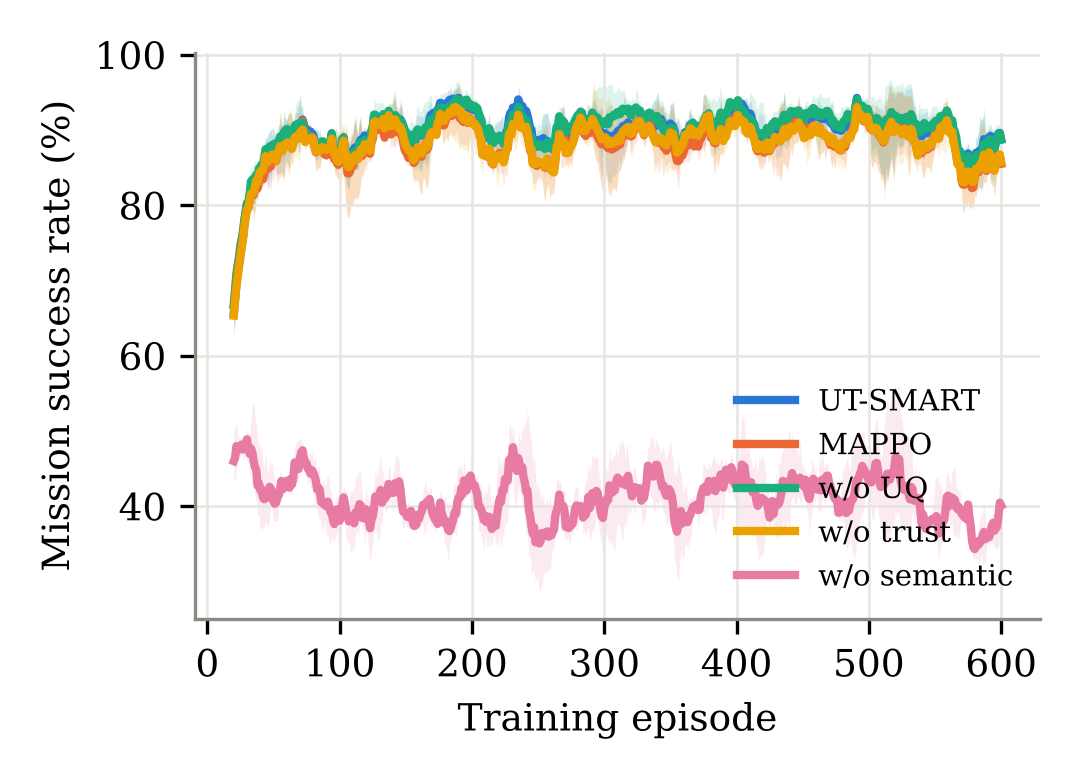
\includegraphics[width=0.92\columnwidth]{fig_convergence.png}
\caption{Training convergence: success rate (20-episode moving average; mean and min--max over 3 seeds) under randomized scenarios.}
\label{fig:conv}
\end{figure}

\subsection{Gateway-Assisted Regime: Density, Fleet Size and Channel}
At the default point ($M=100$, $N=5$, $\sigma=4$~dB, one compromised AUV), UT-SMART completes $98.9\%\pm0.5\%$ of tasks, against 98.4\% for MAPPO, 92.7\% for Greedy-Sem, 33.7\% for Raw-Local and 20.3\% for DE-BR. The two weakest baselines fail for opposite reasons. Raw-Local saturates the acoustic channel: 61\% of its tasks miss their deadline, at 42~J and 166~kbit per task. DE-BR is cheap (5.5~J and 17~kbit per task) but compresses blindly, so 75\% of its results fall below the mission's accuracy floor, which is the cost of optimizing delay and energy alone. Greedy-Sem meets accuracy and deadlines but sends 5.2\% of tasks to the compromised AUV, which corrupts them.

\begin{figure*}[!t]
\centering
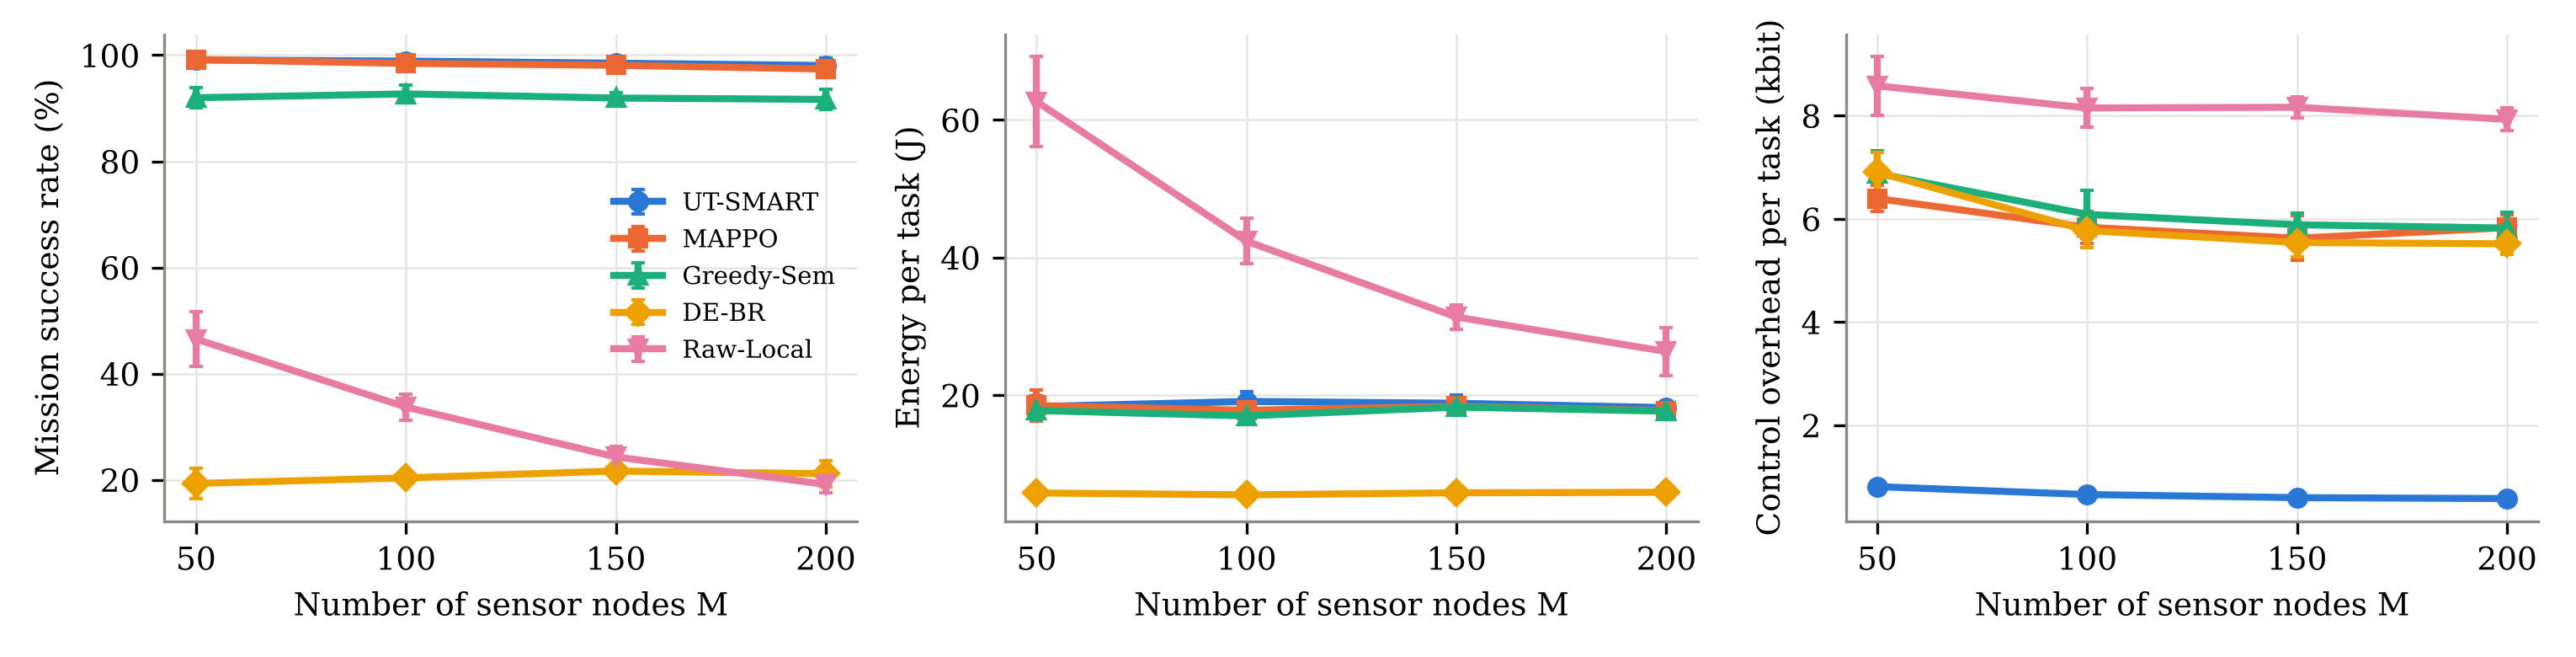
\includegraphics[width=\textwidth]{fig_sensors.png}
\caption{Impact of the number of sensor nodes ($N=5$, gateway-assisted): mission success, energy per task and control overhead per task. Error bars show 95\% confidence intervals over 10 seeds.}
\label{fig:sensors}
\end{figure*}

\begin{figure*}[!t]
\centering
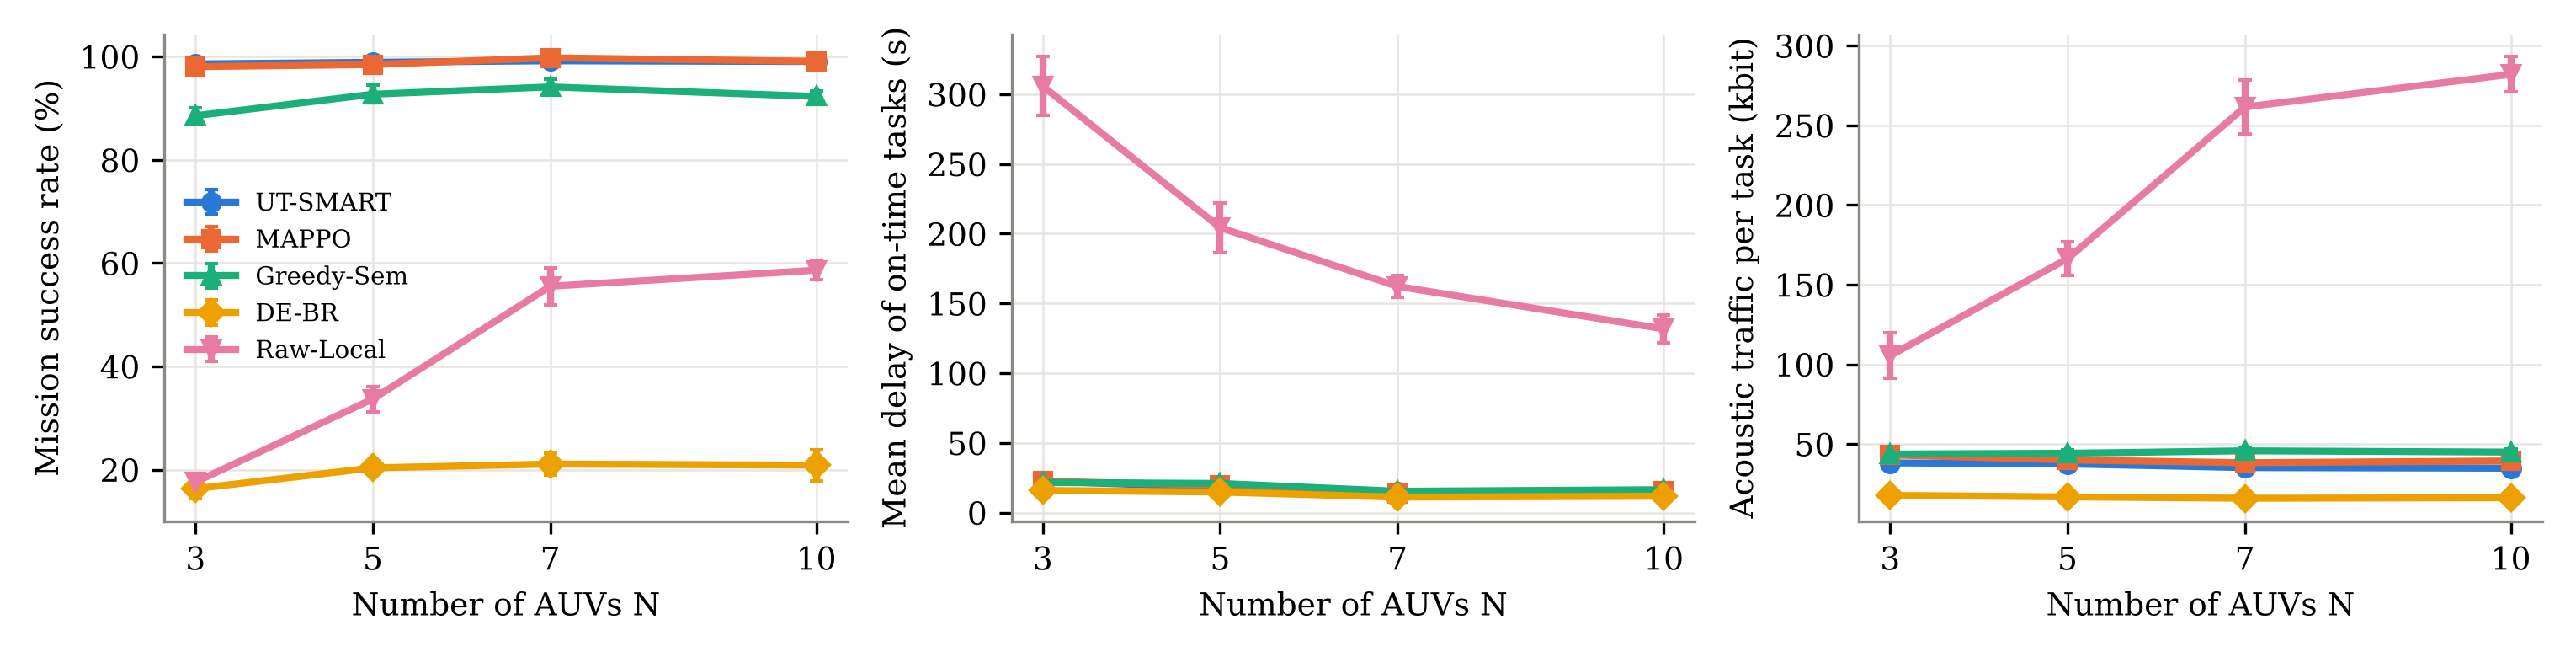
\includegraphics[width=\textwidth]{fig_auvs.png}
\caption{Impact of the number of AUVs ($M=100$, gateway-assisted): mission success, mean delay of on-time tasks and total acoustic traffic per task.}
\label{fig:auvs}
\end{figure*}

Both learned policies learn to send almost all tasks to the gateway, which is accurate and beyond the attacker's reach. In this regime their success rates are statistically indistinguishable ($p=0.43$, paired $t$-test), and UT-SMART's gains are in efficiency (Fig.~\ref{fig:sensors}). Control overhead falls from 5.84 to 0.66~kbit per task ($-89\%$), and the twin's SNR prediction error falls from 3.19 to 2.12~dB ($-34\%$) with one probe per task instead of 9.7. Under load, delay and misses also fall: at $M=200$ the mean delay is 26.1~s against 33.2~s for MAPPO and 34.9~s for Greedy-Sem, and the miss rate is 1.9\% against 2.6\% and 4.0\%. Total acoustic traffic per task is 6\% lower than MAPPO's (37.5 versus 40.0~kbit, $p=0.12$) and 15\% lower than Greedy-Sem's (44.2~kbit). Energy is about 7\% higher than MAPPO's (19.1 versus 17.8~J) because spot checks add uplink traffic. As $N$ grows from 3 to 10, UT-SMART stays at 98.6--99.2\%, whereas Greedy-Sem varies between 88.5\% and 94.1\% (Fig.~\ref{fig:auvs}).

\begin{figure*}[!t]
\centering
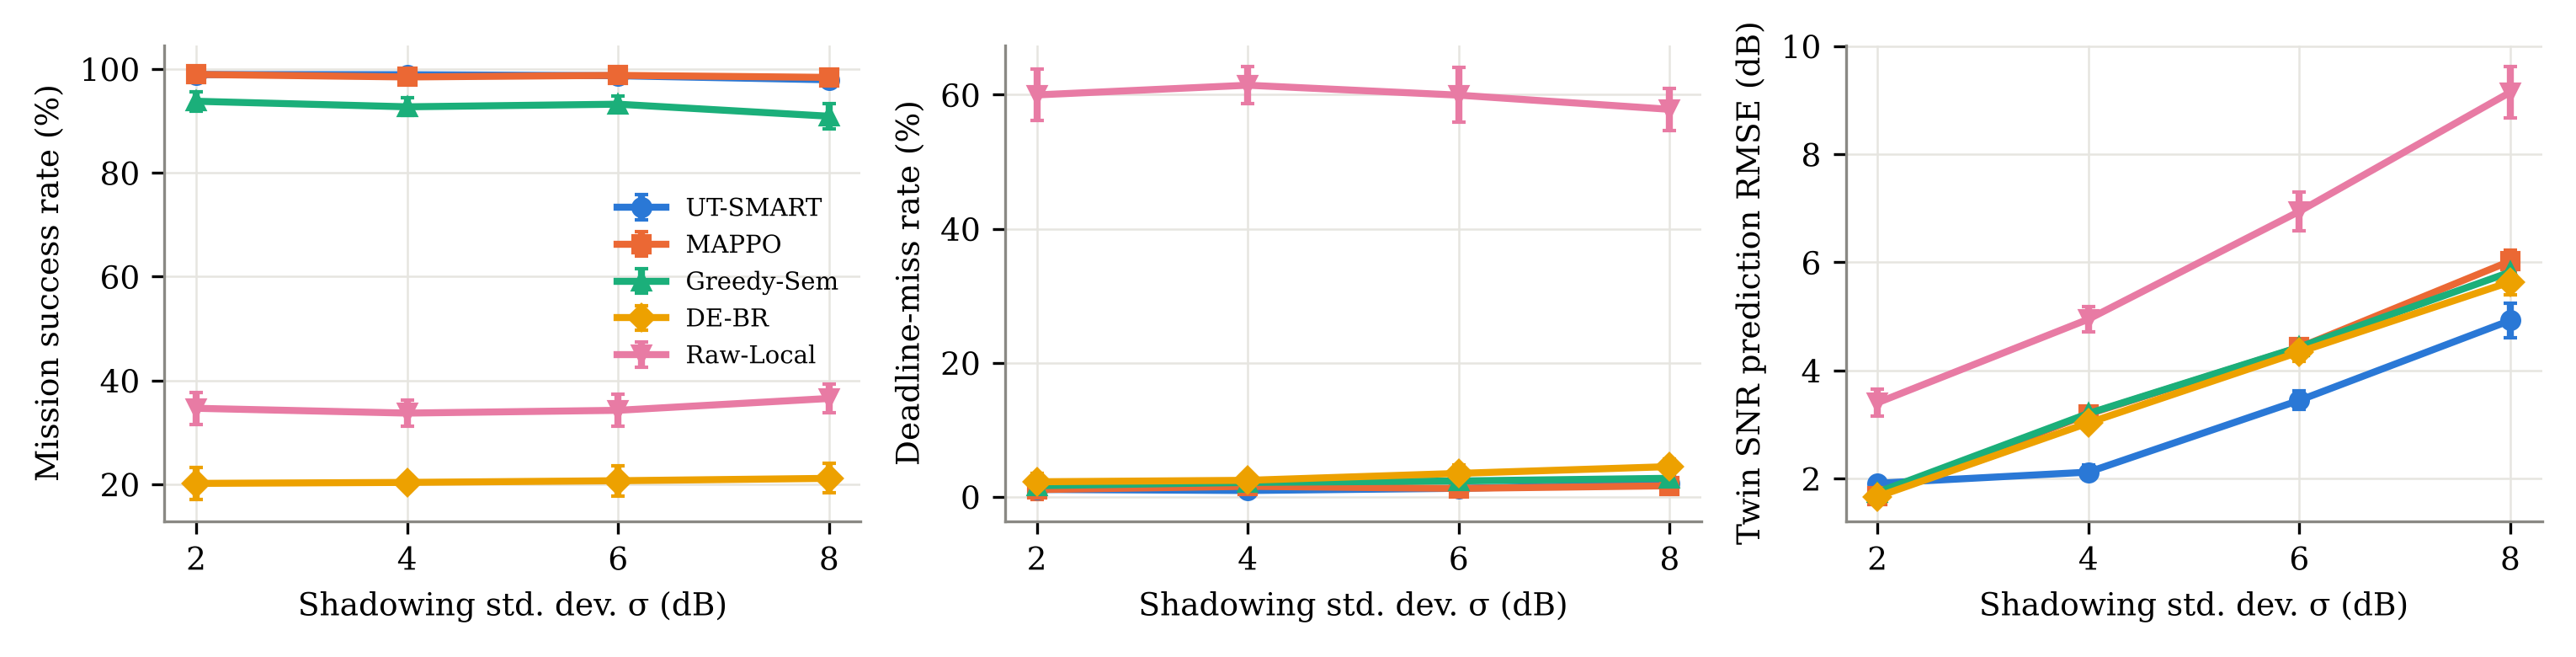
\includegraphics[width=\textwidth]{fig_channel.png}
\caption{Impact of shadowing variability (gateway-assisted): mission success, deadline-miss rate and twin SNR prediction RMSE.}
\label{fig:channel}
\end{figure*}

As the shadowing deviation grows from 2 to 8~dB (Fig.~\ref{fig:channel}), UT-SMART's success stays at or above 97.9\% and its twin error grows more slowly than the baselines' (4.9 versus 6.0~dB at $\sigma=8$~dB). At $\sigma=2$~dB its error is slightly higher (1.91 versus 1.68~dB) because the 2.5-dB probing threshold then exceeds the channel's own variability, so the twin is never probed. The threshold should therefore scale with $\sigma$.

\subsection{AUV-Only Edge Regime and Security}
When the gateway cannot run inference, compromised AUVs can no longer be bypassed, and the learned policies diverge (Fig.~\ref{fig:attack}, $N=10$). With 2 of 10 AUVs compromised, UT-SMART completes 92.7\% of tasks, against 83.7\% for MAPPO, 84.2\% for Greedy-Sem and 84.6\% for UT-SMART without trust. The paired differences are 8.1--9.0 points with $p\le0.007$, and accepted corrupted results fall from 12--13\% to 4.5\%. With 3 compromised AUVs the advantage narrows to 4.1--5.5 points and is not significant over 10 seeds ($p=0.31$--$0.46$); corruption then reaches 13.9\% because the trust estimate needs several spot checks per AUV before it reroutes. In the gateway-assisted regime every learned policy stays at or above 98.8\% at all attack levels, whereas Greedy-Sem drops from 99.0\% to 89.5\%.

\begin{figure*}[!t]
\centering
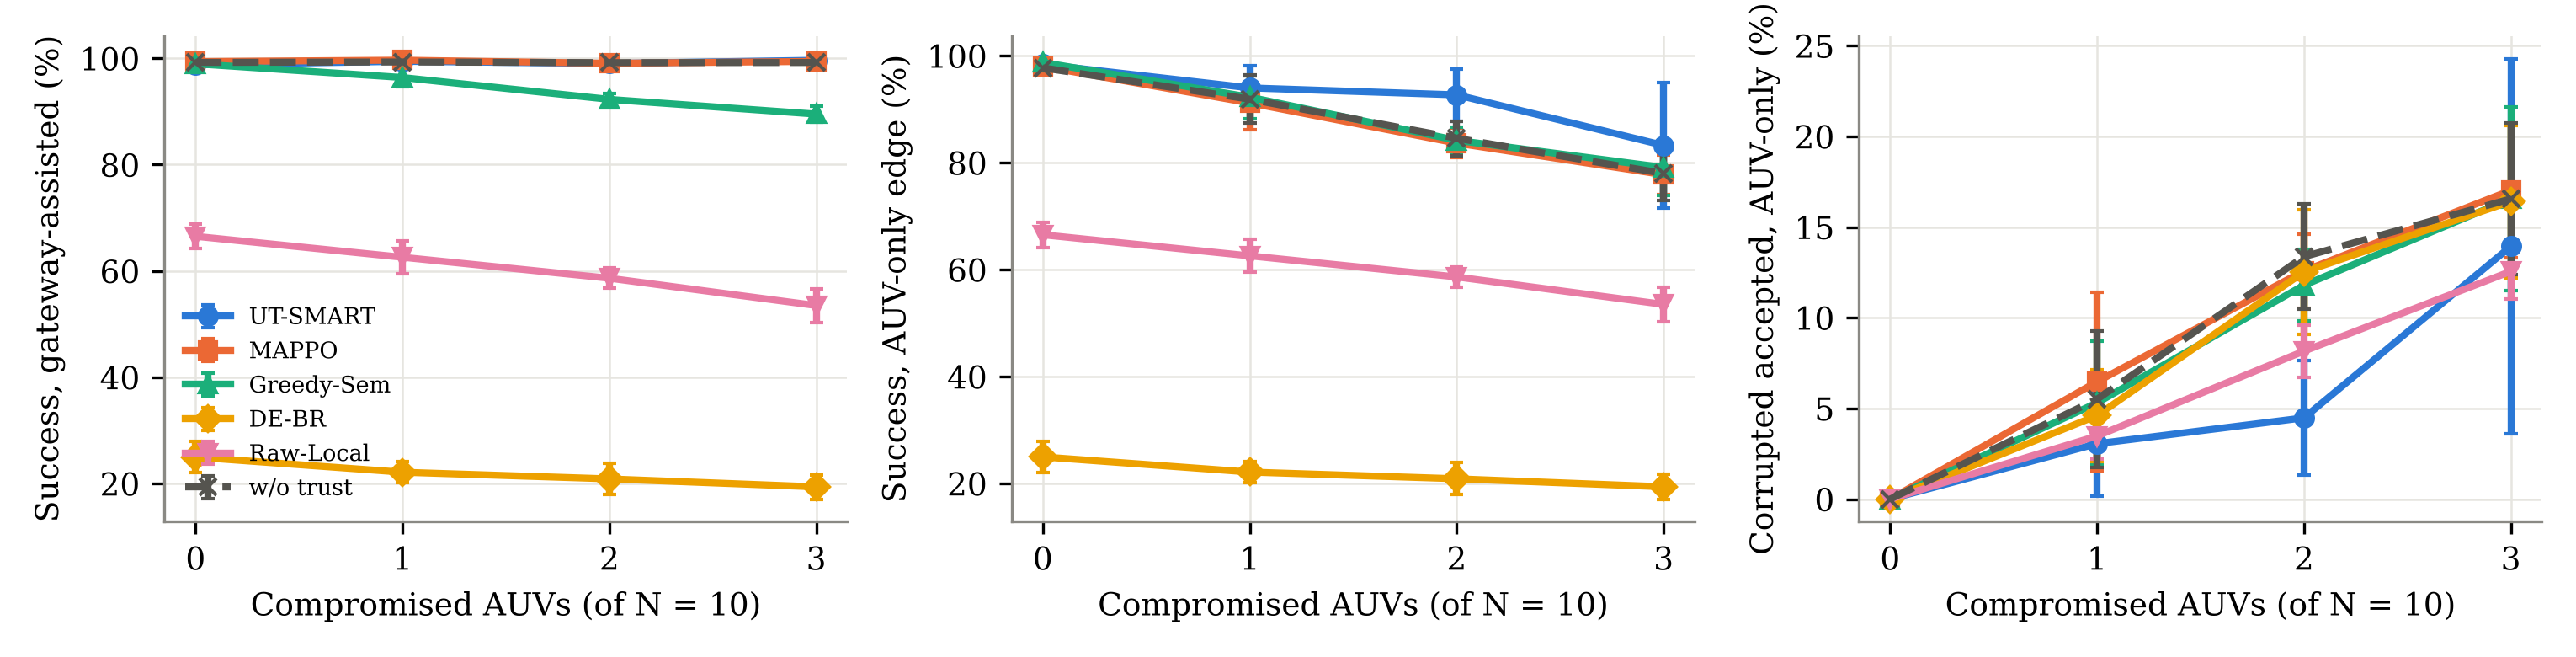
\includegraphics[width=\textwidth]{fig_attack.png}
\caption{Robustness to compromised AUVs ($N=10$): success in the gateway-assisted regime (left) and the AUV-only edge regime (centre), and the share of corrupted results accepted at the AUV-only edge (right). The dashed line is UT-SMART without trust.}
\label{fig:attack}
\end{figure*}

\subsection{Twin Synchronization}
Fig.~\ref{fig:sync} plots twin accuracy against control overhead with the UT-SMART policy held fixed. Periodic synchronization trades one for the other along a curve: shortening the period from 240~s to 20~s lowers the error from 3.55 to 2.72~dB while overhead grows 15-fold, from 1.1 to 16.6~kbit per task. On-demand synchronization with $\tau_s$ between 1.5 and 3~dB reaches 2.12--2.33~dB at about 0.66~kbit per task, which is both more accurate and 25 times cheaper than the 20-s periodic scheme. The gain comes from probing only links that are about to carry data and are uncertain. With $\tau_s=4$~dB ($\ge\sigma$) the twin never probes and the error rises to 3.61~dB. Mission success stays between 98.7\% and 99.2\% at every setting.

\begin{figure}[!t]
\centering
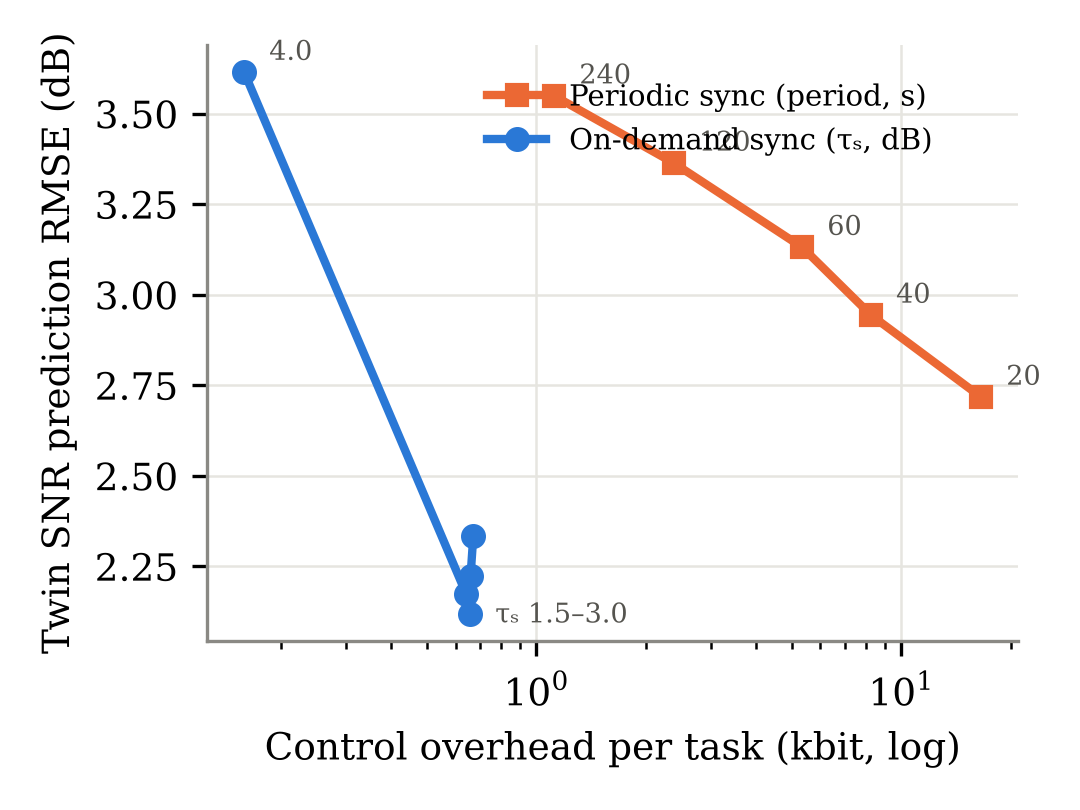
\includegraphics[width=0.92\columnwidth]{fig_sync.png}
\caption{Twin accuracy against control overhead for periodic synchronization (labels: period in s) and on-demand synchronization (labels: threshold $\tau_s$ in dB).}
\label{fig:sync}
\end{figure}

\subsection{Ablation Study}
Table~\ref{tab:ablation} reports each ablation in both regimes ($N=5$, $M=100$, one compromised AUV; mean over 10 seeds, success $\pm$ 95\% confidence interval). Control overhead counts probes and state broadcasts only, and the twin RMSE is measured in the gateway-assisted regime. Four conclusions follow.
\begin{enumerate}
\item \emph{Semantic in-network computing is the foundation:} without it, success collapses to 37\% in both regimes.
\item \emph{Trust gives the largest gain at the AUV-only edge:} it adds 12.5 points ($p=2\times10^{-4}$) and cuts accepted corruption from 12.3\% to 2.2\%, at the cost of 73\% more energy per task (36.2 versus 20.9~J) because tasks are rerouted to farther, trusted AUVs and results are spot-checked.
\item \emph{The uncertainty-aware twin with on-demand synchronization} cuts control overhead about 8-fold and twin error by about a third. Its success gain at the AUV-only edge (4.9--6.6 points) is consistent but not significant over 10 seeds ($p=0.07$--$0.14$).
\item \emph{Event-triggered sharing halves control traffic} (1.40 to 0.66~kbit per task) with no loss of success.
\end{enumerate}
Overall, UT-SMART outperforms MAPPO by 13.4 points ($p=0.003$) at the AUV-only edge and matches it with 89\% less control traffic when the gateway is available.

\begin{table*}[!t]
\centering
\caption{Ablation Study ($N=5$, $M=100$, One Compromised AUV, 10 Seeds)}
\label{tab:ablation}
\begin{tabular}{@{}lcccccc@{}}
\toprule
Variant & \shortstack{Success,\\gateway (\%)} & \shortstack{Success,\\AUV-only (\%)} & \shortstack{Corrupted,\\AUV-only (\%)} & \shortstack{Control\\(kbit/task)} & \shortstack{Twin\\RMSE (dB)} & \shortstack{Energy, AUV-\\only (J/task)}\\
\midrule
\textbf{UT-SMART (full)} & $\mathbf{98.9\pm0.5}$ & $\mathbf{89.2\pm4.7}$ & \textbf{2.2} & \textbf{0.66} & \textbf{2.12} & 36.2\\
w/o uncertainty (mean twin, periodic sync) & $98.4\pm0.6$ & $82.6\pm5.1$ & 9.7 & 5.14 & 3.15 & 29.2\\
w/o on-demand sync (periodic 60 s) & $98.9\pm0.4$ & $84.3\pm6.8$ & 5.5 & 5.35 & 3.13 & 37.2\\
w/o trust & $99.1\pm0.5$ & $76.7\pm5.0$ & 12.3 & 0.66 & 2.12 & 20.9\\
w/o event-triggered sharing (20 s periodic) & $99.1\pm0.5$ & $86.7\pm6.1$ & 3.1 & 1.40 & 2.16 & 37.3\\
w/o semantic computing (raw only) & $36.7\pm2.9$ & $36.7\pm2.9$ & 6.0 & 0.71 & 5.63 & 51.5\\
MAPPO (none of the above) & $98.4\pm0.8$ & $75.8\pm5.6$ & 11.5 & 5.84 & 3.19 & 20.8\\
\bottomrule
\end{tabular}
\end{table*}

\subsection{Discussion and Limitations}\label{sec:disc}

\emph{When does each mechanism matter?} The results show a clear division of labour. Semantic compression is necessary in every setting, because the acoustic channel cannot carry raw sensing data at mission rates. When a trustworthy, accurate gateway is reachable, the best policy is simply to use it; learning then adds little success over a well-designed MARL baseline, and the twin and event-triggered mechanisms pay off as an 89\% cut in control traffic. When computation must stay on vehicles, which is the normal case for deep, long-range or covert missions, trust-aware assignment becomes decisive. We therefore recommend evaluating underwater edge-intelligence schemes in both regimes, because a gateway-rich setting alone can hide security weaknesses.

\emph{Limitations:} First, the evaluation is simulation only. The channel follows standard Thorp--Urick models with AR(1) shadowing and Markov outages, but it omits multipath delay spread, Doppler and MAC-layer collisions beyond the shared FIFO; porting UT-SMART to Aqua-Sim-NG or DESERT and to sea-trial traces~\cite{song2025dtna,xu2025stgr} is the next step. Second, the accuracy--compression curve $\delta_k$ and the encoder costs are modelling assumptions rather than measurements of a trained detector; calibrating them with an underwater detector (e.g., a YOLO-style detector with a MobileNetV3 backbone) on sonar and optical datasets would ground the accuracy constraint. Third, the per-link Kalman twin is cheap and calibrated but ignores spatial correlation between links; temporal graph or Transformer predictors could share information across links and vehicles, provided they also output calibrated uncertainty, for example through deep ensembles~\cite{lakshminarayanan2017ensembles}. Fourth, AUV trajectories are fixed and the learner uses one-step advantages, so joint trajectory control and longer-horizon credit assignment for queue effects remain open. Fifth, the attackers follow fixed strategies; adaptive attackers that behave well under spot checks, colluding AUVs and jamming would stress the trust model further, and with 3 of 10 AUVs compromised our improvement was no longer significant. Finally, at the AUV-only edge, trust-driven rerouting raises energy per task by about 73\%, which motivates an energy-aware trust threshold.

%======================================================================
\section{Conclusion}\label{sec:concl}
We presented UT-SMART, an edge-intelligence framework for connected AUVs that jointly decides semantic compression at the sensor and inference placement across AUVs and the surface gateway under mission-specific deadline, accuracy and VoI requirements. It combines a Bayesian digital twin that knows its own uncertainty and synchronizes on demand, constrained multi-agent PPO over the twin's what-if predictions, Beta-reputation trust inside the policy and event-triggered state sharing. In simulations over 10 seeds, UT-SMART completed 98.9\% of tasks with a gateway available, matching a MAPPO baseline while using 89\% less control traffic and a 34\% more accurate twin. Without the gateway and with one compromised AUV, it completed 89.2\% of tasks against 75.8\% for MAPPO and cut accepted corrupted results from 11.5\% to 2.2\%. Future work will calibrate the accuracy model with real underwater detectors, move to packet-level simulators and sea-trial traces, and extend the policy to trajectory control and adaptive adversaries.

\section*{Code and Data Availability}
The simulator, training and evaluation scripts, trained models and per-seed results will be released in a public repository upon acceptance.

%======================================================================
\begin{thebibliography}{28}

\bibitem{yang2021survey}
Y. Yang, Y. Xiao, and T. Li, ``A survey of autonomous underwater vehicle formation: Performance, formation control, and communication capability,'' \textit{IEEE Commun. Surveys Tuts.}, vol. 23, no. 2, pp. 815--XXXX, 2nd Quart. 2021.

\bibitem{dai2022survey}
M. Dai, Y. Li, P. Li, Y. Wu, L. Qian, B. Lin, and Z. Su, ``A survey on integrated sensing, communication, and computing networks for smart oceans,'' \textit{J. Sens. Actuator Netw.}, vol. 11, no. 4, Art. no. 70, 2022, doi: 10.3390/jsan11040070.

\bibitem{lin2025madac}
C. Lin, Y. Zhang, G. Han, C. Lu, S. Zhu, and S. Wang, ``Multiple autonomous underwater vehicles-assisted data collection in 6G-driven underwater wireless networks based on software-defined MARL,'' \textit{IEEE Trans. Intell. Transp. Syst.}, vol. 26, no. 10, pp. 17928--XXXX, Oct. 2025.

\bibitem{song2025dtna}
S. Song, B. Huangfu, J. Guo, J. Liu, J. Cui, and X. Shen, ``A digital twin-based intelligent network architecture for underwater acoustic sensor networks,'' \textit{IEEE Trans. Mobile Comput.}, vol. 24, no. 9, pp. 8196--XXXX, Sep. 2025.

\bibitem{xu2025stgr}
C. Xu, S. Song, X. Wu, G. Han, M. Pan, G. Xu, and J.-H. Cui, ``A high reliable routing protocol based on spatial-temporal graph model for multiple unmanned underwater vehicles network,'' \textit{IEEE Trans. Mobile Comput.}, vol. 24, no. 5, pp. 4434--XXXX, May 2025.

\bibitem{shu2026offload}
J. Shu, Y. Guo, Z. Chen, Z. Cui, Y. Chen, L. Zhao, and X. Chen, ``AUV-assisted task offloading in underwater acoustic sensor networks with end-edge-cloud collaboration: A game-theoretic approach,'' \textit{IEEE Trans. Mobile Comput.}, vol. 25, no. 11, pp. 20691--XXXX, Nov. 2026.

\bibitem{stojanovic2007capacity}
M. Stojanovic, ``On the relationship between capacity and distance in an underwater acoustic communication channel,'' \textit{ACM SIGMOBILE Mobile Comput. Commun. Rev.}, vol. 11, no. 4, pp. 34--43, 2007.

\bibitem{mao2017mec}
Y. Mao, C. You, J. Zhang, K. Huang, and K. B. Letaief, ``A survey on mobile edge computing: The communication perspective,'' \textit{IEEE Commun. Surveys Tuts.}, vol. 19, no. 4, pp. 2322--2358, 4th Quart. 2017.

\bibitem{pang2020sagin}
Y. Pang, D. Wang, D. Wang, L. Guan, C. Zhang, and M. Zhang, ``A space-air-ground integrated network assisted maritime communication network based on mobile edge computing,'' in \textit{Proc. IEEE World Congr. Services (SERVICES)}, 2020, doi: 10.1109/SERVICES48979.2020.00060.

\bibitem{chen2025ios}
H. Chen, Y. Wen, Y. Huang, C. Xiao, and Z. Sui, ``Edge computing enabling Internet of Ships: A survey on architectures, emerging applications, and challenges,'' \textit{IEEE Internet Things J.}, vol. 12, no. 2, pp. 1509--XXXX, Jan. 2025.

\bibitem{su2020maritime}
X. Su, L. Meng, and J. Huang, ``Intelligent maritime networking with edge services and computing capability,'' \textit{IEEE Trans. Veh. Technol.}, vol. 69, no. 11, pp. 13606--XXXX, Nov. 2020.

\bibitem{wu2024inc}
D. Wu, Z. Wang, H. Pan, H. Yao, T. Mai, and S. Guo, ``In-network computing empowered mobile edge offloading architecture for Internet of Things,'' \textit{IEEE Trans. Services Comput.}, vol. 17, no. 6, pp. 3817--XXXX, Nov./Dec. 2024.

\bibitem{hong2024cnc}
Z. Hong, X. Qiu, J. Lin, W. Chen, Y. Yu, H. Wang, S. Guo, and W. Gao, ``Intelligence-endogenous management platform for computing and network convergence,'' \textit{IEEE Netw.}, 2024, doi: 10.1109/MNET.2023.3321529.

\bibitem{ahmad2026survey}
I. Ahmad, R. Narmeen, U. A. Mughal, L. Yang, J. Li, Y. Alkhrijah, and M. K. Khan, ``A comprehensive survey on cybersecurity challenges and defenses for integrated air, ground, and underwater autonomous vehicle systems,'' \textit{IEEE Commun. Surveys Tuts.}, vol. 28, pp. 6512--XXXX, 2026.

\bibitem{zhang2025dfxtna}
P. Zhang, X. He, and J. Yu, ``A distributed fixed-time neurodynamic algorithm and its application in multi-autonomous underwater vehicle collaborative escorting,'' \textit{IEEE Trans. Netw. Sci. Eng.}, vol. 12, no. 5, pp. 4140--XXXX, Sep./Oct. 2025.

\bibitem{lowe2017maddpg}
R. Lowe, Y. Wu, A. Tamar, J. Harb, P. Abbeel, and I. Mordatch, ``Multi-agent actor-critic for mixed cooperative-competitive environments,'' in \textit{Proc. Adv. Neural Inf. Process. Syst. (NeurIPS)}, vol. 30, 2017, pp. 6379--6390.

\bibitem{das2019tarmac}
A. Das, T. Gervet, J. Romoff, D. Batra, D. Parikh, M. Rabbat, and J. Pineau, ``TarMAC: Targeted multi-agent communication,'' in \textit{Proc. 36th Int. Conf. Mach. Learn. (ICML)}, PMLR vol. 97, 2019, pp. 1538--1546.

\bibitem{huang2020droo}
L. Huang, S. Bi, and Y.-J. A. Zhang, ``Deep reinforcement learning for online computation offloading in wireless powered mobile-edge computing networks,'' \textit{IEEE Trans. Mobile Comput.}, vol. 19, no. 11, pp. 2581--2593, Nov. 2020.

\bibitem{kang2017neurosurgeon}
Y. Kang, J. Hauswald, C. Gao, A. Rovinski, T. Mudge, J. Mars, and L. Tang, ``Neurosurgeon: Collaborative intelligence between the cloud and mobile edge,'' in \textit{Proc. 22nd Int. Conf. Archit. Support Program. Lang. Oper. Syst. (ASPLOS)}, Xi'an, China, 2017, pp. 615--629.

\bibitem{shao2022taskoriented}
J. Shao, Y. Mao, and J. Zhang, ``Learning task-oriented communication for edge inference: An information bottleneck approach,'' \textit{IEEE J. Sel. Areas Commun.}, vol. 40, no. 1, pp. 197--211, Jan. 2022.

\bibitem{xie2021deepsc}
H. Xie, Z. Qin, G. Y. Li, and B.-H. Juang, ``Deep learning enabled semantic communication systems,'' \textit{IEEE Trans. Signal Process.}, vol. 69, pp. 2663--2675, 2021.

\bibitem{altman1999cmdp}
E. Altman, \textit{Constrained Markov Decision Processes}. Boca Raton, FL, USA: CRC Press, 1999.

\bibitem{lakshminarayanan2017ensembles}
B. Lakshminarayanan, A. Pritzel, and C. Blundell, ``Simple and scalable predictive uncertainty estimation using deep ensembles,'' in \textit{Proc. Adv. Neural Inf. Process. Syst. (NeurIPS)}, vol. 30, 2017, pp. 6402--6413.

\bibitem{josang2002beta}
A. J{\o}sang and R. Ismail, ``The Beta reputation system,'' in \textit{Proc. 15th Bled Electron. Commerce Conf.}, 2002, pp. 41--55.

\bibitem{schulman2017ppo}
J. Schulman, F. Wolski, P. Dhariwal, A. Radford, and O. Klimov, ``Proximal policy optimization algorithms,'' 2017, \textit{arXiv:1707.06347}.

\bibitem{yu2022mappo}
C. Yu, A. Velu, E. Vinitsky, J. Gao, Y. Wang, A. Bayen, and Y. Wu, ``The surprising effectiveness of PPO in cooperative multi-agent games,'' in \textit{Proc. Adv. Neural Inf. Process. Syst. (NeurIPS) Datasets Benchmarks Track}, 2022.

\bibitem{tessler2019rcpo}
C. Tessler, D. J. Mankowitz, and S. Mannor, ``Reward constrained policy optimization,'' in \textit{Proc. Int. Conf. Learn. Represent. (ICLR)}, New Orleans, LA, USA, 2019.

\bibitem{achiam2017cpo}
J. Achiam, D. Held, A. Tamar, and P. Abbeel, ``Constrained policy optimization,'' in \textit{Proc. 34th Int. Conf. Mach. Learn. (ICML)}, PMLR vol. 70, 2017, pp. 22--31.

\end{thebibliography}

\vspace{-20pt}
\begin{IEEEbiographynophoto}{Manimurugan Shanmuganathan}
(Senior Member, IEEE) is with the Faculty of Computers and Information Technology, University of Tabuk, Tabuk, Saudi Arabia. He received the Ph.D. degree from Anna University, Chennai, India, in 2012. He has authored numerous research papers in leading journals, including the IEEE Internet of Things Journal, the IEEE Transactions on Intelligent Transportation Systems, and the IEEE Transactions on Consumer Electronics. His research interests include artificial intelligence of things, medical image processing, deep learning, cyber-physical systems for intelligent transportation, and secure edge intelligence.
\end{IEEEbiographynophoto}

\vspace{-20pt}
\begin{IEEEbiographynophoto}{P. Karthikeyan}
received the B.E. degree in computer science and engineering from Anna University, Chennai, India, in 2005, the M.E. degree in computer science and engineering from Anna University, Coimbatore, India, in 2009, and the Ph.D. degree from Anna University, Chennai, in 2018. He was a Postdoctoral Research Fellow with the Department of Computer Science and Information Engineering, National Chung Cheng University, Taiwan, where he contributed to national projects supported by the National Science and Technology Council, Taiwan. He is currently an Associate Professor with the School of Computer Science and Engineering, RV University, Bengaluru, India. His research interests include cloud computing, edge computing, and applied deep learning.
\end{IEEEbiographynophoto}

\vspace{-20pt}
\begin{IEEEbiographynophoto}{Ahmed Aljuhani}
is with the Faculty of Computers and Information Technology, University of Tabuk, Tabuk, Saudi Arabia. He has published widely in venues including the IEEE Transactions on Vehicular Technology, the IEEE Internet of Things Journal, and the IEEE Transactions on Consumer Electronics. His research interests include cybersecurity, intrusion detection, Internet of Things and industrial IoT security, blockchain, digital twins, federated edge intelligence, and explainable artificial intelligence.
\end{IEEEbiographynophoto}

\vspace{-20pt}
\begin{IEEEbiographynophoto}{Alireza Jolfaei}
(Senior Member, IEEE) received the Ph.D. degree in applied cryptography from Griffith University, Gold Coast, Australia. He is an Associate Professor of Networking and Cyber Security with the College of Science and Engineering, Flinders University, Adelaide, Australia. He was previously a faculty member with Macquarie University and Federation University Australia, and with Temple University, Philadelphia, PA, USA. He has published over 100 peer-reviewed papers. He is a Distinguished Speaker of the ACM, Chair of the Security and Privacy Technical Committee of the IEEE Consumer Technology Society, and an Associate Editor of the IEEE Transactions on Intelligent Transportation Systems. He received the IEEE Australia Council Award for his research paper published in the IEEE Transactions on Information Forensics and Security. His main research interest is cyber-physical systems security, including the security of intelligent transportation and industrial control systems.
\end{IEEEbiographynophoto}

\end{document}
